\documentclass{beamer}
\setbeamertemplate{footline}[page number]
\date{}
\author{}
\institute{}

%%%%%%% Put these names back in the final version 
%\\Aswathy Rajendra Kurup\\Meenu Ajith}
%\institute{Department of Electrical and Computer Engineering\\The University of New Mexico}
\setbeamercovered{transparent}
\usepackage{setspace}
\usepackage{array}
\usepackage[T1]{fontenc}
\usepackage{graphicx}
\usepackage{amsmath}
\usepackage{amsfonts}
\usepackage{amssymb}
\usepackage{makeidx}
\usefonttheme{serif}
\usepackage{multirow}
\usepackage{booktabs} 
\usepackage{rotating}
\usepackage{color}
\usepackage{float}
\usepackage[latin1]{inputenc}
\usepackage[english]{babel}
\usepackage{amsmath}
\usepackage{amsfonts}
\usepackage{eurosym}
\usepackage{rotating}
\usepackage{multicol}
\usepackage{pythonhighlight}
\usepackage[normalem]{ulem}
\newcommand{\ba}{{\bf a}}
\newcommand{\bb}{{\bf b}}
\newcommand{\bc}{{\bf c}}
\newcommand{\bd}{{\bf d}}
\newcommand{\be}{{\bf e}}
\newcommand{\bbf}{{\bf f}}
\newcommand{\bg}{{\bf g}}
\newcommand{\bh}{{\bf h}}
\newcommand{\bi}{{\bf i}}
\newcommand{\bk}{{\bf k}}
\newcommand{\bl}{{\bf l}}
\newcommand{\bm}{{\bf m}}
\newcommand{\bn}{{\bf n}}
\newcommand{\bo}{{\bf o}}
\newcommand{\bp}{{\bf p}}
\newcommand{\bq}{{\bf q}}
\newcommand{\br}{{\bf r}}
\newcommand{\bs}{{\bf s}}
\newcommand{\bt}{{\bf t}}
\newcommand{\bu}{{\bf u}}
\newcommand{\bv}{{\bf v}}
\newcommand{\bw}{{\bf w}}
\newcommand{\bx}{{\bf x}}
\newcommand{\by}{{\bf y}}
\newcommand{\bz}{{\bf z}}

\newcommand{\bA}{{\bf A}}
\newcommand{\bB}{{\bf B}}
\newcommand{\bC}{{\bf C}}
\newcommand{\bE}{{\bf E}}
\newcommand{\bG}{{\bf G}}
\newcommand{\bH}{{\bf H}}
\newcommand{\bI}{{\bf I}}
\newcommand{\bK}{{\bf K}}
\newcommand{\bL}{{\bf L}}
\newcommand{\bM}{{\bf M}}
\newcommand{\bO}{{\bf O}}
\newcommand{\bQ}{{\bf Q}}
\newcommand{\bR}{{\bf R}}
\newcommand{\bS}{{\bf S}}
\newcommand{\bT}{{\bf T}}
\newcommand{\bV}{{\bf V}}
\newcommand{\bW}{{\bf W}}
\newcommand{\bX}{{\bf X}}
\newcommand{\bY}{{\bf Y}}
\newcommand{\bZ}{{\bf Z}}
\newcommand\uptocnt{\stackrel{\mathclap{\normalfont\mbox{c}}}{\propto}}
\newcommand{\bpt}{{\bf pt}}
\newcommand{\bpl}{{\bf pl}}
\newcommand{\bdp}{{\bf dp}}
\newcommand{\btemp}{{\bf temp}}

\newcommand{\bmu}{{\boldsymbol \mu}}
\newcommand{\bSigma}{{\boldsymbol \Sigma}}
\newcommand{\bsigma}{{\boldsymbol \sigma}}
\newcommand{\bvarPhi}{{\boldsymbol \varPhi}}
\newcommand{\bvarphi}{{\boldsymbol \varphi}}
\newcommand{\bPhi}{{\boldsymbol \Phi}}
\newcommand{\bdelta}{{\boldsymbol \delta}}
\newcommand{\bZero}{{\bf 0}}
\newcommand{\bOne}{{\bf 1}}
\newcommand{\balpha}{{\boldsymbol \alpha}}
\newcommand{\bAlpha}{{\boldsymbol A}}
\newcommand{\btheta}{{\boldsymbol \theta}}

\newcommand{\softmax}{\text{softmax}}
\newcommand{\diag}{\text{diag}}
\newcommand{\sinc}{\mathrm{sinc}}
\newcommand{\argmin}{\mathop{\mathrm{argmin}}}
\newcommand{\infl}{\eta}
\newcommand{\Ind}{\mathrm{I}}
\newcommand{\Real}{\mathbb R}
\newcommand{\Intg}{\mathbb Z}
\newcommand{\Complex}{\mathbb C}
\newcommand{\Natural}{\mathbb N}
\newcommand{\Fourier}[1]{\mathcal{F} \{#1\}}
%\newcommand{\ii}{\mathbbm{i}}
\newcommand{\bphi}{\boldsymbol{\mathit{\phi}}}

\newcommand{\hs}{\hspace{2pt}}
\newcommand{\sign}{\text{sign}}
\author{Manel Mart\'inez-Ram\'on\\Meenu Ajith\\Aswathy Rajendra Kurup}

\usetheme{Madrid}
\usecolortheme{beaver}
\usepackage{tikz}
\usetikzlibrary{fit,arrows,calc,positioning}
\usepackage{listings}
\usepackage{xcolor}
\usepackage{emerald} 
\usepackage[T1]{fontenc} 
\usepackage{verbatim}
\usepackage{graphicx}
\usepackage{epsfig}
\usepackage{psfrag}
\usepackage[english]{babel}
\usepackage{listings}
\usepackage{courier}
\usepackage{color}
 \usepackage{vwcol} 
 \usepackage[english]{babel} % To obtain English text with the blindtext package
\usepackage{blindtext}
\definecolor{codegreen}{rgb}{0,0.6,0}
\definecolor{codegray}{rgb}{0.5,0.5,0.5}
\definecolor{codepurple}{rgb}{0.58,0,0.82}
\definecolor{backcolour}{rgb}{0.95,0.95,0.92}

\lstdefinestyle{mystyle}{
  backgroundcolor=\color{backcolour},   commentstyle=\color{codegreen},
  keywordstyle=\color{magenta},
  numberstyle=\tiny\color{codegray},
  stringstyle=\color{codepurple},
  basicstyle=\ttfamily\footnotesize,
  breakatwhitespace=false,         
  breaklines=true,                 
  captionpos=b,                    
  keepspaces=true,                 
  numbers=left,                    
  numbersep=5pt,                  
  showspaces=false,                
  showstringspaces=false,
  showtabs=false,                  
  tabsize=2
}
\lstset{style=mystyle}

%% Stuff for movies

% %\newcommand{\bt}{{\bf t}}
% \newcommand{\br}{{\bf r}}
% \newcommand{\bs}{{\bf s}}
% \newcommand{\by}{{\bf y}}
% \newcommand{\bz}{{\bf z}}
% \newcommand{\bx}{{\bf x}}
% \newcommand{\bw}{{\bf w}}
% \newcommand{\be}{{\bf e}}
% \newcommand{\bbf}{{\bf f}}
% \newcommand{\bb}{{\bf b}}
% \newcommand{\bd}{{\bf d}}
% \newcommand{\bA}{{\bf A}}
% \newcommand{\bB}{{\bf B}}
% \newcommand{\bL}{{\bf L}}
% \newcommand{\bM}{{\bf M}}

% \newcommand{\bC}{{\bf C}}
% \newcommand{\bI}{{\bf I}}
% \newcommand{\bK}{{\bf K}}
% \newcommand{\bk}{{\bf k}}
% \newcommand{\bT}{{\bf T}}
% \newcommand{\bV}{{\bf V}}
% \newcommand{\bW}{{\bf W}}
% \newcommand{\bX}{{\bf X}}
% \newcommand{\bY}{{\bf Y}}
% \newcommand{\bZ}{{\bf Z}}
% \newcommand{\bm}{{\bf m}}
% \newcommand{\bpt}{{\bf pt}}
% \newcommand{\bpl}{{\bf pl}}
% \newcommand{\bdp}{{\bf dp}}
% \newcommand{\btemp}{{\bf temp}}
% \newcommand{\bl}{{\bf l}}
% \newcommand{\bu}{{\bf u}}
% \newcommand{\bmu}{{\boldsymbol \mu}}
% \newcommand{\bSigma}{{\boldsymbol \Sigma}}
% \newcommand{\bLambda}{{\boldsymbol \Lambda}}

% \newcommand{\bsigma}{{\boldsymbol \sigma}}
% \newcommand{\bvarphi}{{\boldsymbol \varPhi}}
% \newcommand{\btheta}{{\boldsymbol \theta}}
% \newcommand{\bZero}{{\bf 0}}
% \newcommand{\balpha}{{\boldsymbol \alpha}}
% \newcommand{\bpi}{{\boldsymbol \pi}}
% \newcommand{\bxi}{{\boldsymbol \xi}}
% \newcommand{\bdelta}{{\boldsymbol \delta}}
\lstset{
	language=Python,
	basicstyle=\footnotesize\ttfamily\color{black},
	commentstyle = \footnotesize\ttfamily\color{red},
	keywordstyle=\footnotesize\ttfamily\color{blue},
	stringstyle=\footnotesize\ttfamily\color{black},
%	columns=fixed,
%	numbers=left,    
	numberstyle=\tiny,
	stepnumber=1,
	numbersep=5pt,
	tabsize=1,
	extendedchars=true,
	breaklines=true,            
	frame=b,         
	showspaces=false,
	showtabs=true,
	xleftmargin=6pt,
	framexleftmargin=6pt,
	framexrightmargin=2pt,
	framexbottommargin=4pt,
	showstringspaces=false      
}

\lstloadlanguages{
         Python
}

%\graphicspath{ {./images/} }  % Figures path - used in graphicx

%\selectcolormodel{cmyk}

\mode<presentation>

\newcommand{\dred}{darkred!90!black}
\newcommand{\written}{\ECFJD\textcolor{cyan!50!white}}
\newcommand{\hlight}{\textcolor{\dred}}
\newcommand{\Ex}{\textcolor{\dred}{Ex. }}

% remove navigation symbols in full screen mode
\setbeamertemplate{navigation symbols}{}  
\setbeamertemplate{blocks}[rounded][shadow=false]
\setbeamercolor{note page}{fg=black}

\setbeamercolor{title}{fg=\dred}
\setbeamercolor{frametitle}{fg=white}
\setbeamercolor{frametitle}{bg=\dred}
\setbeamercolor{structure}{fg=black,bg=white}
\setbeamercolor{background canvas}{bg=white,fg=black}
\setbeamercolor{normal text}{fg=black,bg=white}
\setbeamercolor{item}{fg=red!80!black,bg=white!}
\addtobeamertemplate{block begin}{\setbeamercolor{block title}{fg=white,bg=\dred}
\setbeamercolor{block body}{fg=white,bg=gray}}{}


\title{4. Convolutional neural networks}
\subtitle{4.1. Elements of the convolutional neural network}

\addtobeamertemplate{frametitle}{}


\begin{document}

\maketitle

\begin{frame}{Introduction}
\begin{itemize}
    \item The basic NN in Module 1 extracts features of a pattern through a nonlinear representation in a higher dimensional space. 
    \item Next layers represent features with a higher level of abstraction.
    \item In the last layer, the features produce representations of the input pattern that can be linearly classified. 

    \item The core of the NN is the affine transformation $\bW^\top \bx +\bb$ plus a nonlinear activation. 

    \item This is a global transformation that does not have local properties. 

    \item Local feature representation capabilities are needed in, for example, images. 
\end{itemize}
\end{frame}

\begin{frame}{Overall structure}
\begin{itemize}
\item Several convolutional blocks, including convolutions, pooling and activation layers.
\item A fully connected block, consisting of a standard MLP. 
\end{itemize}
\begin{center}
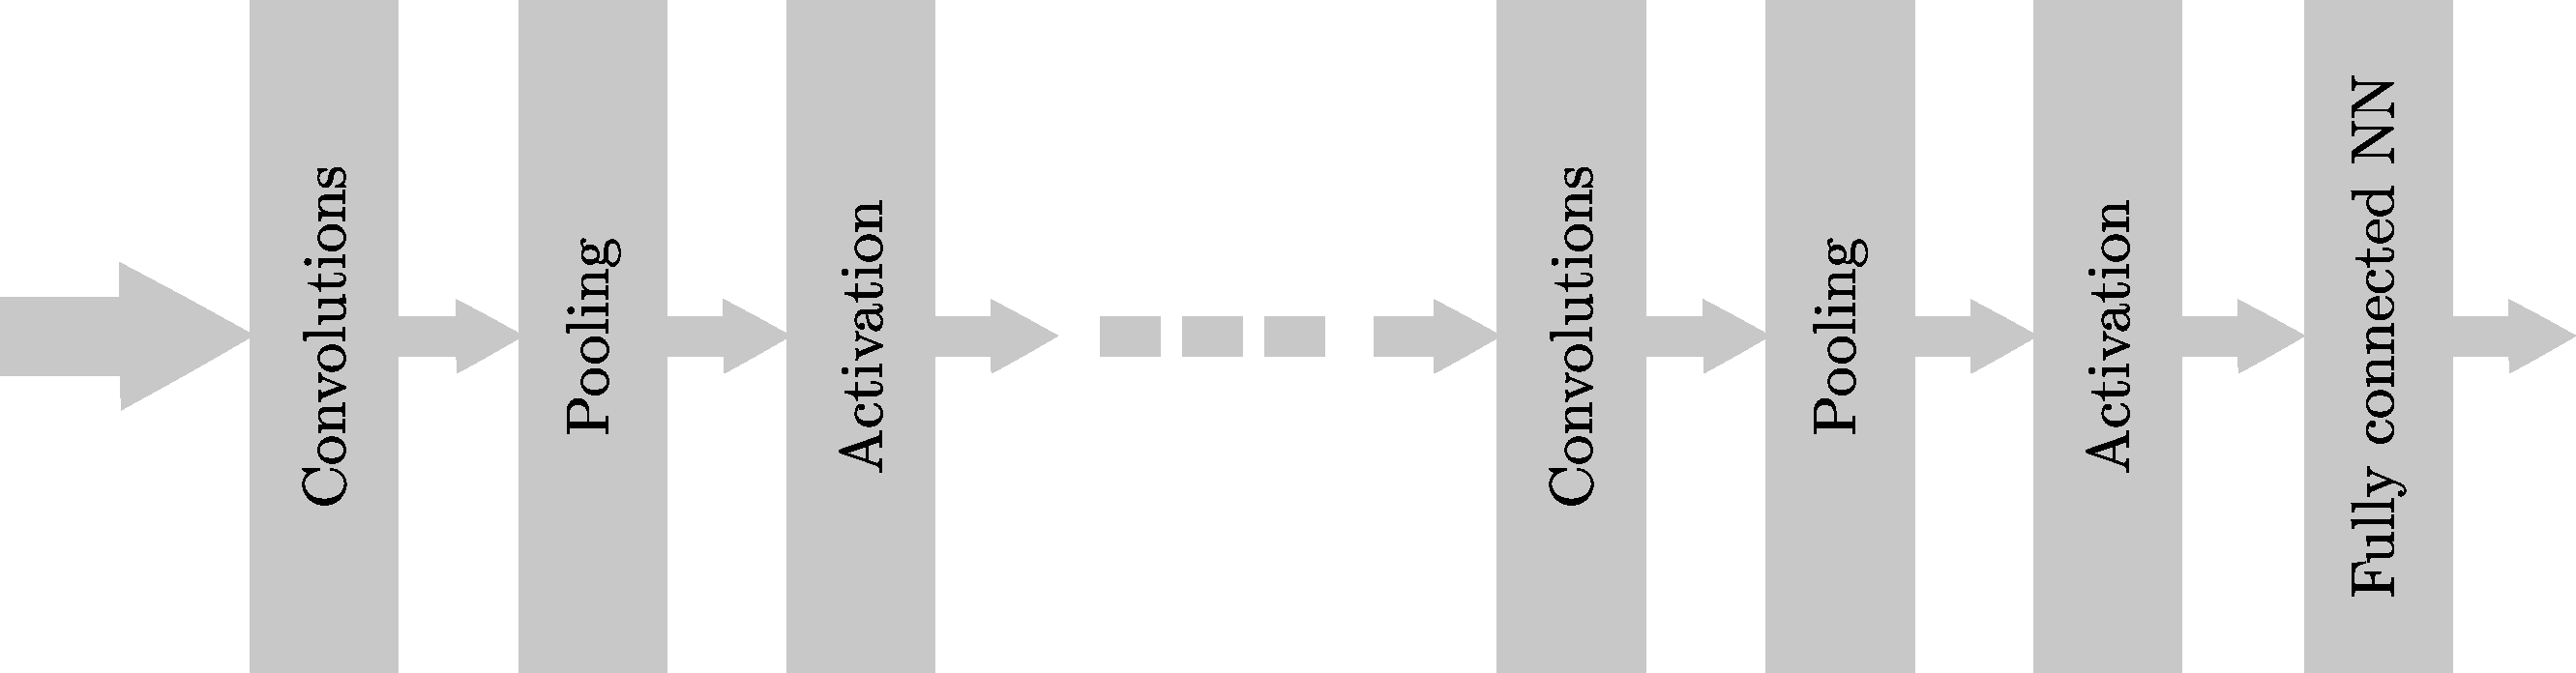
\includegraphics[scale=0.2]{Module 4 (CNN)/pics/CNN.pdf}
\end{center}
\begin{itemize}
    \item The output can contain a softmax (multiclass classification) or linear activation. 
\end{itemize}
\end{frame}
\begin{frame}{Review of the convolution concept}
\begin{itemize}
    \item In one dimension, the discrete convolution is defined as
    \begin{equation}\label{eq:convolution}
    \left(f*g\right)[n] = \sum_{m=-\infty}^\infty f[m]g[n-m]
\end{equation}
\end{itemize}
\begin{center}
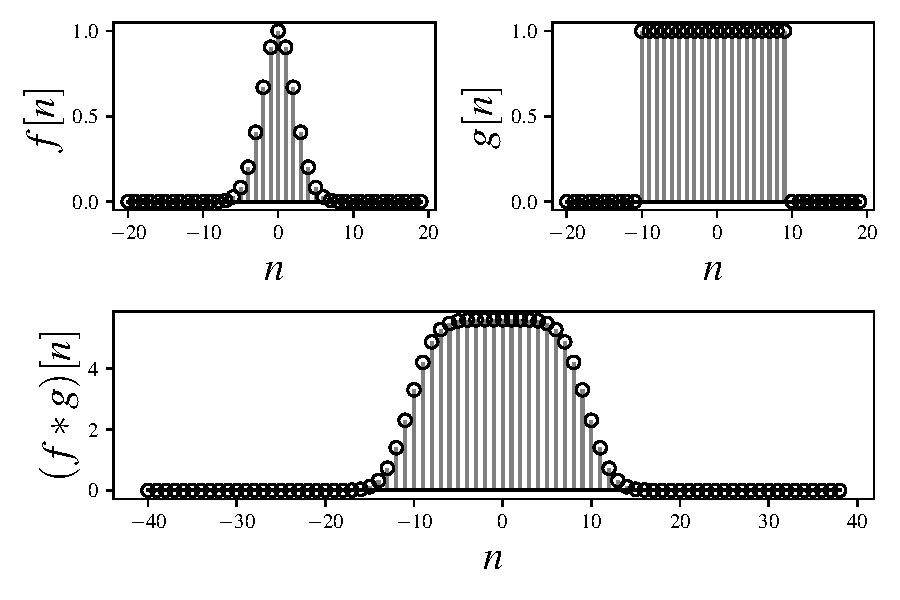
\includegraphics[scale=0.3]{Module 4 (CNN)/pics/ex_convolution_lpfilter.pdf}
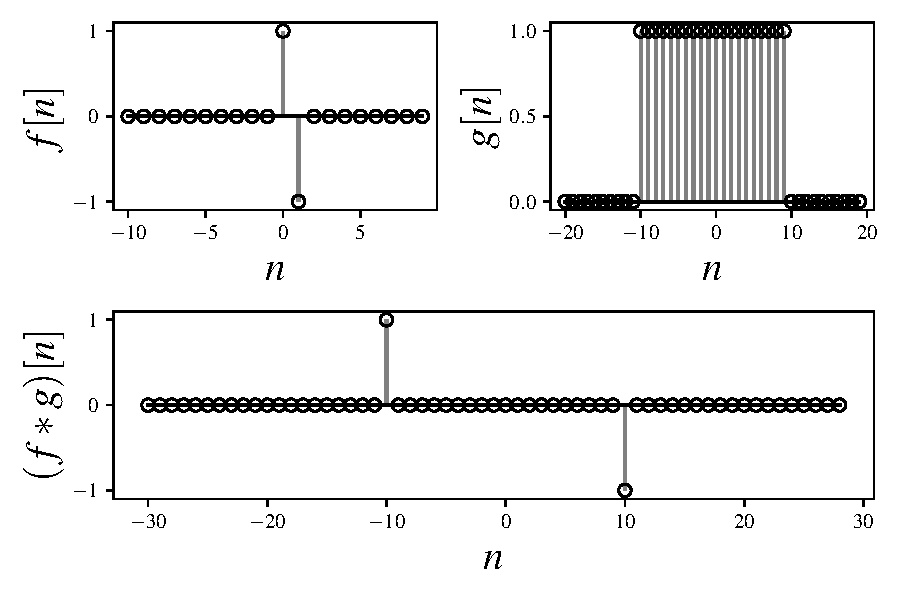
\includegraphics[scale=0.3]{Module 4 (CNN)/pics/ex_convolution_derivative.pdf}
\end{center}
\begin{itemize}
    \item At point n, the convolution is the sum of products of one signal times the other one shifted n positions and reversed.
\end{itemize}
\end{frame}

\begin{frame}{Convolutions in 2 dimensions}
\begin{itemize}
    \item The extension to 2 dimensions is immediate. 
    \begin{equation}\label{eq:2Dconvolution}
    \left(\bI*\bW\right)[m,n] = \sum_{p=0}^{M_W-1} \sum_{q=0}^{N_W-1} \bW[p,q]\bI[m+p,n+q]
\end{equation}
\end{itemize} 
\begin{multicols*}{2}
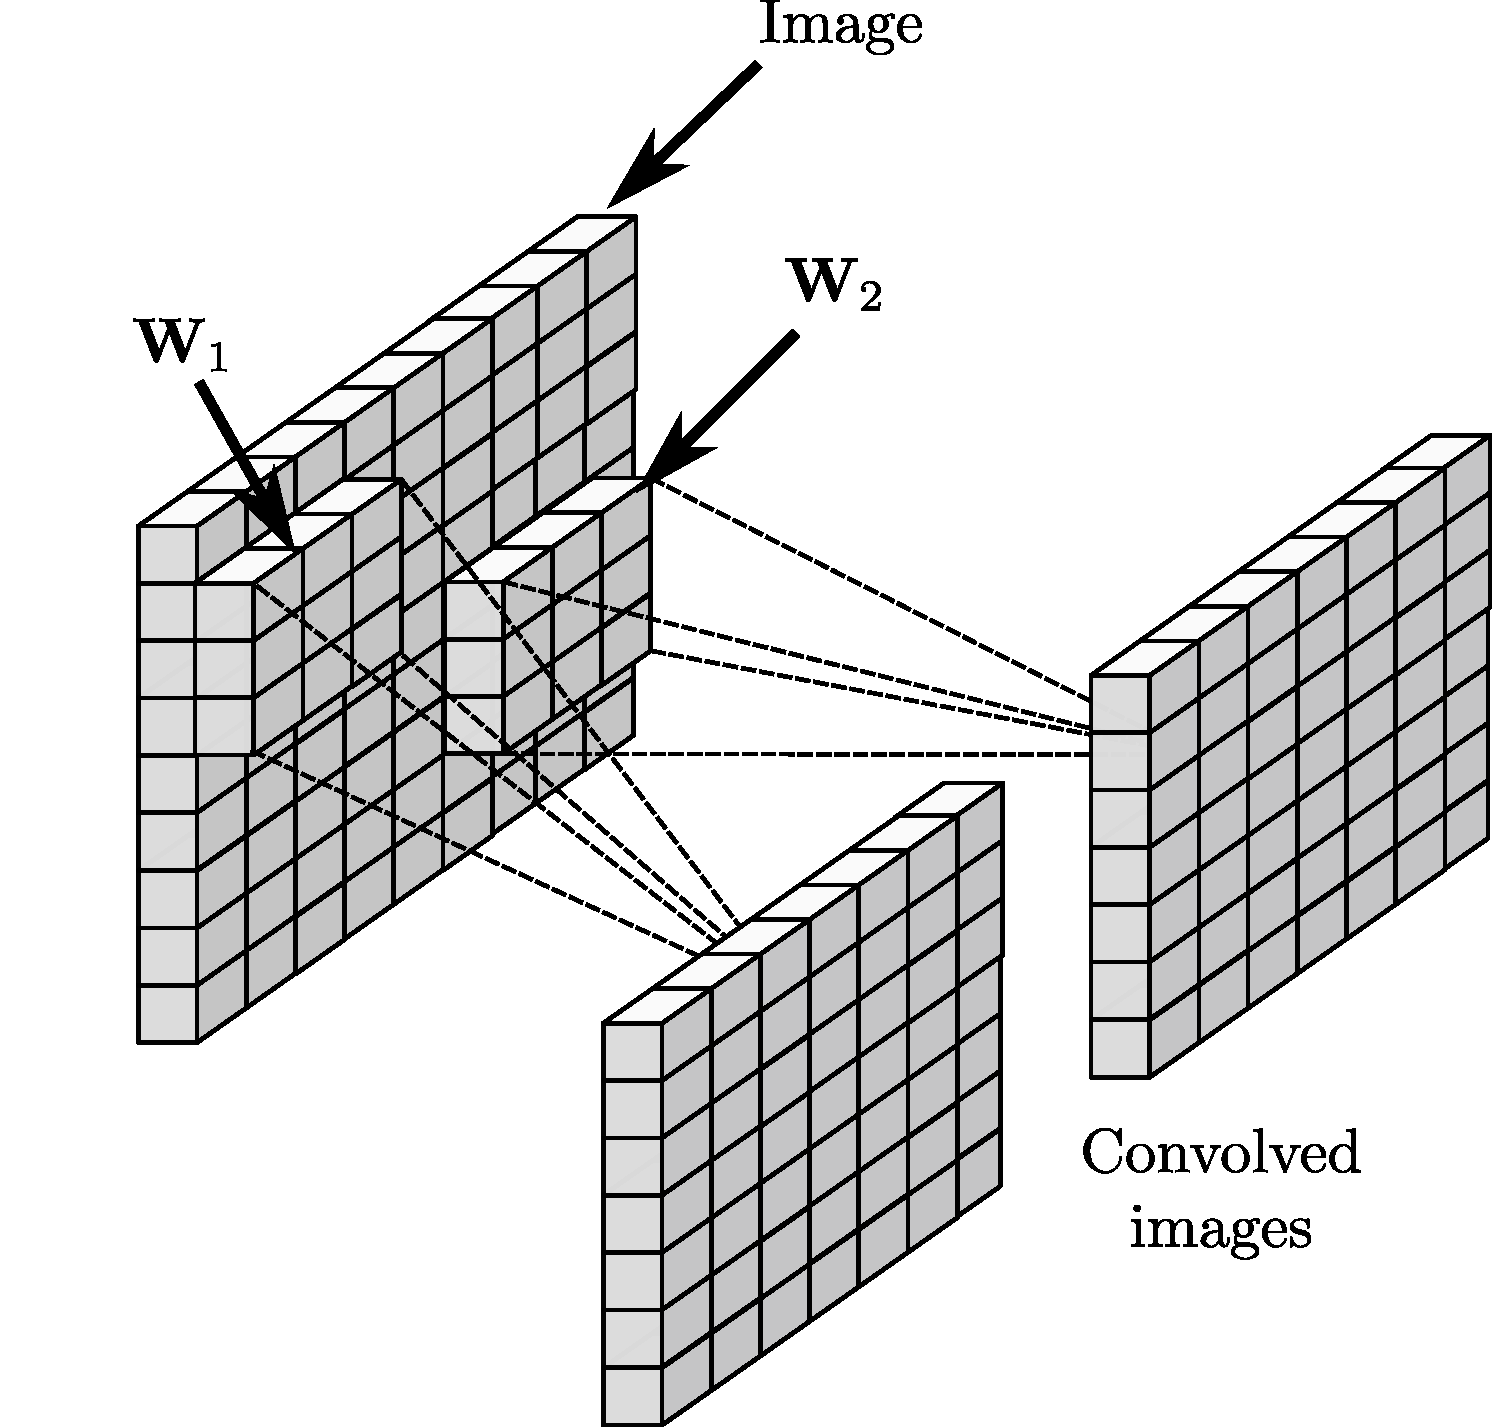
\includegraphics[scale=0.2]{Module 4 (CNN)/pics/CONVOLUTION1.pdf}
\begin{tiny}Image convolved with kernels $\bW_1$ and $\bW_2$.\end{tiny}

\columnbreak

\vspace*{1pt}

\begin{itemize}
\item Image $\bI$ of dimension $M_I\times N_I$.
\item \emph{Convolution kernel} $\bW$: array of dimensions $M_W\times N_W$.
\item Dimensions of the resulting array: $M_I-M_W+1 \times N_I-N_W +1$. 
\end{itemize}
\end{multicols*}
\end{frame}

\begin{frame}{What is a convolutional layer for?}

\begin{itemize}
\item Problem: detect an object or shape in an image regardless of its position.

\item Its exact rotation, and scale will also be issues, but let's not mind this for now.

\item The position of the object must not be relevant, so each extracted  feature must receive information from all pixels.
\end{itemize}
\end{frame}
\begin{frame}{Example of a convolution}
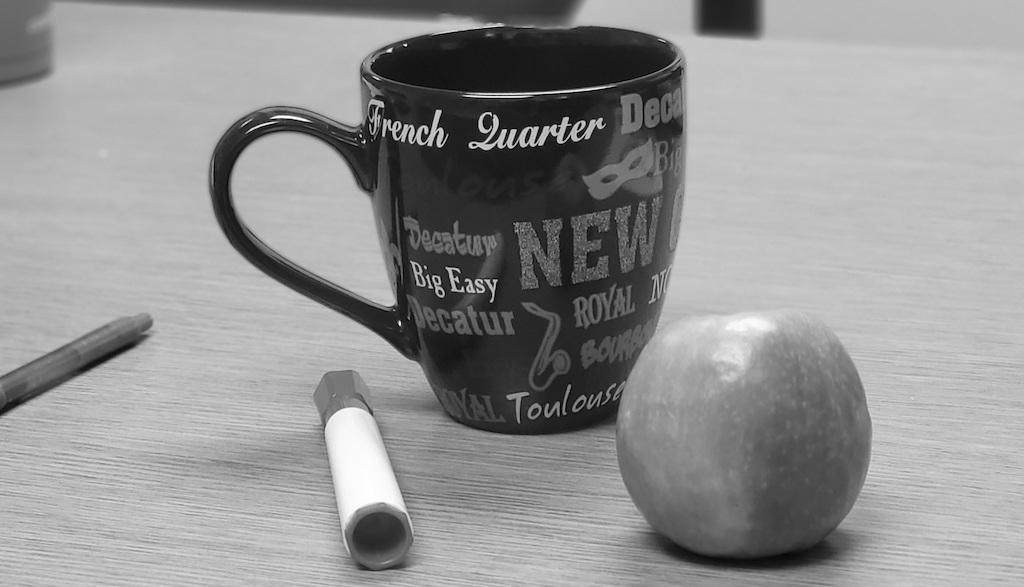
\includegraphics[width=0.45\textwidth]{Module 4 (CNN)/pics/I.jpg}
    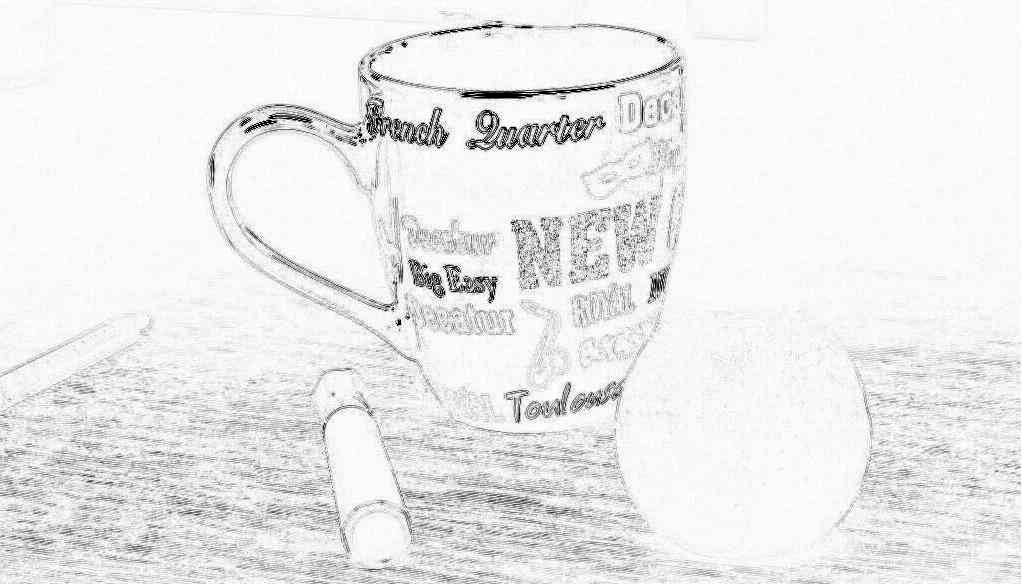
\includegraphics[width=0.45\textwidth]{Module 4 (CNN)/pics/O_processed.png}
    {Example of the convolution of an image with a convolution kernel designed to enhance the edges of the image. }
\begin{itemize}
    \item The image has been convolved with the kernel 
    \begin{equation}
    \bW =
    \left( 
    \begin{array}{rrr}
         -1 & -1 & -1  \\
         -1 & 8 & -1  \\
         -1 & -1 & -1  \\
    \end{array}
    \right)
\end{equation}

\end{itemize}
\end{frame}

\begin{frame}{Padding}
    \begin{itemize}
        \item  The convolution crops the image. The convolution dimensions are $$M_I-M_W+1 \times N_I-N_W +1$$ 
    \item The pixels at the edge of the image are seen only when the convolution kernel touches the edge of the image. 
    \item If we add $p$ rows/columns of zeros, the output dimensions are
\begin{equation}
    \left( M_I - M_W + p  + 1 \right)\times\left( N_I - N_W + p  + 1 \right)
\end{equation}
\item If $p/2$ rows are added to each side of the input image so the number of rows of the convolved image does not change: 
 $$M_I+p - M_W+1 = M_I$$ 
 $$\frac{p}{2} = \frac{M_W-1}{2}$$
hence $M_W$ must be odd. 
\end{itemize}
\end{frame}

\begin{frame}{Padding}
    \begin{center}
    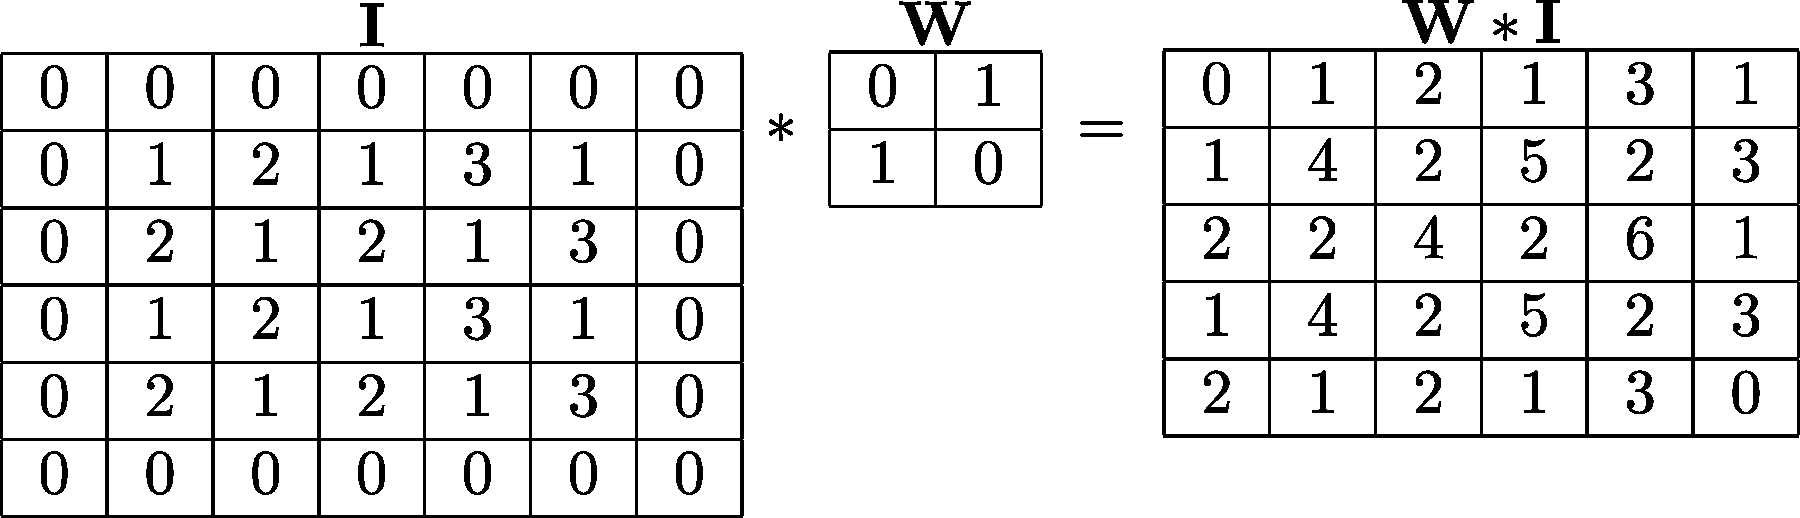
\includegraphics[scale=0.35]{Module 4 (CNN)/pics/conv_example2.pdf}
    \end{center}
    Example of zero padding . The input, with dimensions $5\times4$, is padded with 2 zeros in each dimension. The output has dimensions $6 \times 5$.  For a convolution kernel of dimensions $3\times3$, the output will have dimensions $5 \times 4$.
\end{frame}

\begin{frame}{Stride}
\begin{itemize}
\item Defines the amount of overlap between areas covered by the convolution kernel.
\item A stride $s=1$ means that two adjacent values of the convolution have been obtained by shifting one position (in either direction) the convolution kernel (no stride).

\item A stride of  $s$ means that between two steps of the convolution in either direction, the kernel is shifted $s$ positions.

\item As a consequence, the output has lower dimensions. For a convolution with padding $p$ and stride $s$, the output dimensions will be
\begin{equation}\label{eq:conv_dimensions}
\left\lfloor\frac{M_I+p-M_w+s}{s}\right\rfloor\times
\left\lfloor\frac{N_I+p-N_w+s}{s}\right\rfloor
\end{equation}

    \end{itemize}
\end{frame}

\begin{frame}{Stride}
\begin{center}
    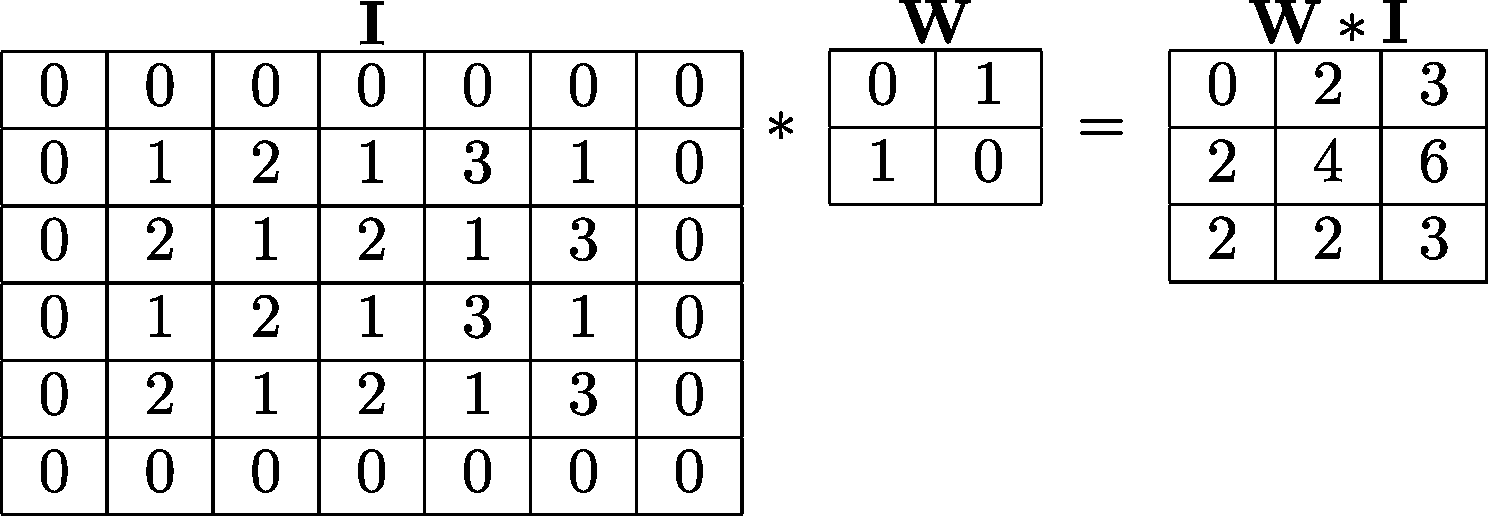
\includegraphics[scale=0.35]{Module 4 (CNN)/pics/conv_stride.pdf}
\end{center}
 Example of padding and stride, where $p=2$ and $s=2$. The resulting dimensions are $3\times 3$.
\end{frame}


\begin{frame}{Pooling}

\begin{itemize}
\item Pooling is applied to the output to reduce the size of the convolution in a controlled way.
\item This reduces the complexity of the structure. 
\item This is desired to limit the computational cost and the overfitting.
\item The operation selects a square window with $q$ pixels and maps them into a scalar.
\item Next, the window is shifted to one or more positions and the operation is repeated. 
\item The most usual ones are \emph{max pooling}, which selects the maximum value of the window, and \emph{average pooling}. 
\end{itemize}
\end{frame}


\begin{frame}{Channels}

\begin{multicols}{2}
\begin{center}
    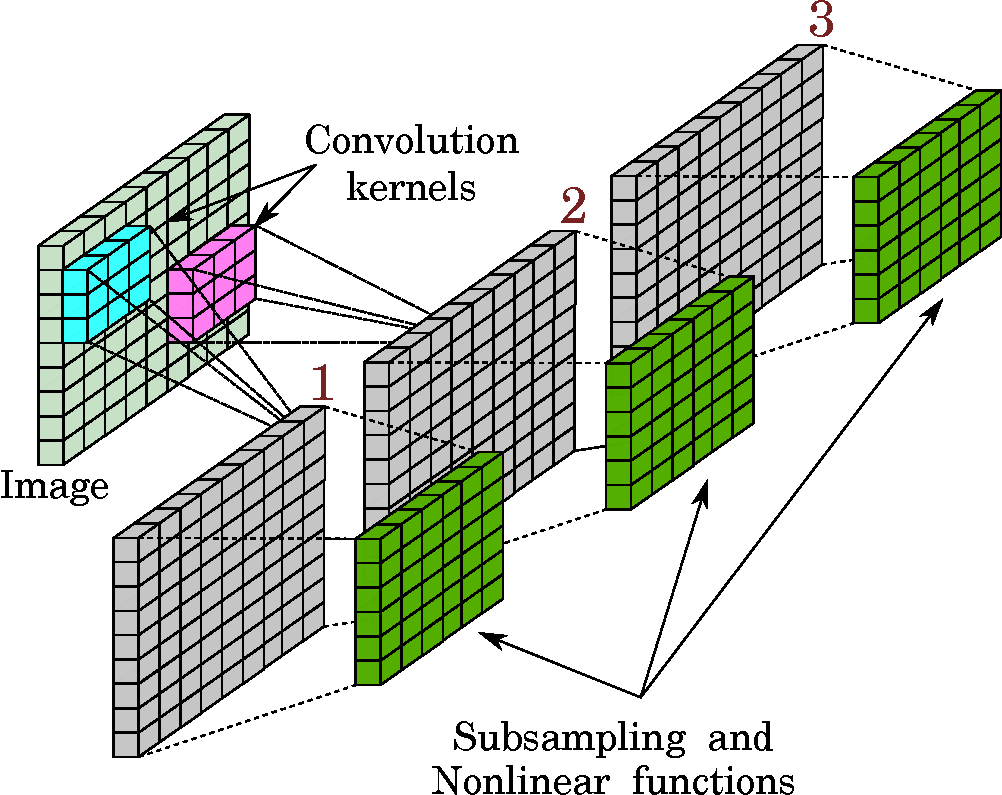
\includegraphics[scale=0.3]{Module 4 (CNN)/pics/f5.4.pdf}
\end{center}
\columnbreak

\begin{itemize}
\item The paths from the original image to the convolution outputs are calles \emph{channels}. 

\item We can apply the convolution again to all the channel outputs. 

\item An image with $L$ channels  can be mapped to an image with $M$ channels.  
\item Each channel is a linear combination of convolutions. 
\end{itemize}  
\end{multicols}
\end{frame}

\begin{frame}{Formulation of the CNN convolution}
\begin{itemize}
    \item Assume an RGB image $\bI$ with dimensions $[C_I, M_I, N_I]$, $C_I=3$ corresponding to the three color channels.
    \item Every color of the image is convolved with several convolution kernels. 
    \item Define $\bW_{j,k}$, $0\leq j \leq C_I-1$ as the collection of convolution kernels that convolve input channel $\bI_j$ and transform it into  channel $\bZ_k$. Then 
    \begin{equation}
    \bZ_k = \sum_{j=0}^{C_I-1} \bW_{j,k} * \bI_j + \bB_k 
\end{equation}
where a bias array $\bB_k$ is added after the convolution.
\end{itemize}
\end{frame}

\begin{frame}{Formulation of the CNN convolution}
\begin{multicols}{2}
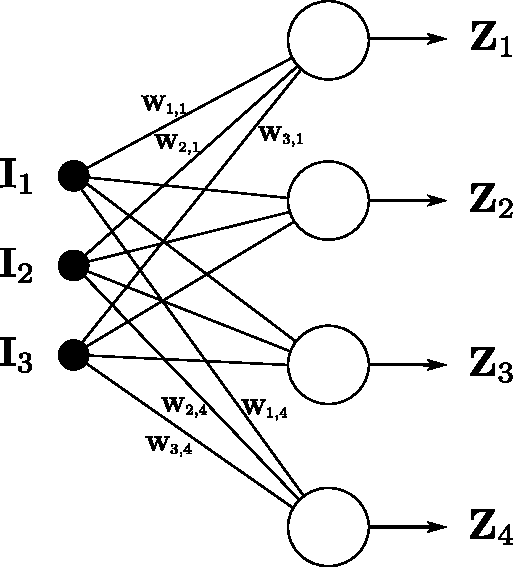
\includegraphics[scale=0.5]{Module 4 (CNN)/pics/Conv_rep.pdf}

Convolution layer  with 3 input channels and 4 output channels. 

\columnbreak 

\begin{itemize}
    \item Each output channel is expressed as


 \begin{equation}\nonumber
    \bZ_k = \sum_{j=0}^{C_I-1} \bW_{j,k} * \bI_j + \bB_k 
\end{equation}
\item where convolution kernel ${\bf W}_{j,k}$ connects input channel $j$ with output channel $k$. 
\item Bias matrices not represented. \item Outputs ${\bf Z}_k$ are applied an activation and a pooling.  
\end{itemize}

\end{multicols}
\end{frame}



\begin{frame}{Formulation of the CNN convolution}
\begin{itemize}
    \item In a convolutional neural network, one convolutional layer computes the above operation with all the output channels of the previous layer as follows
    \begin{equation}
\begin{split}
    &\bZ^{(l)}_k[n] = \sum_{j=0}^{C^{(l-1)}-1} \bW^{(l)}_{j,k} * \bH^{(l-1)}_j[n] + \bB^{(l)}_k \\
    &\bH^{(l)}_k[n] = \bvarphi\left( \bZ^{(l)}_k[n] \right)\\
    &0\leq k \leq C^{(l)}-1
\end{split}
\end{equation}
\item Here $\bvarphi(\cdot)$ represents a pooling and a nonlinear activation, while padding and stride are assumed to be applied to the image and to the convoution kernels. 
\end{itemize}
\end{frame}

\begin{frame}{Interpretation as neural connectivity}
\begin{multicols}{2}
    
\begin{center}
    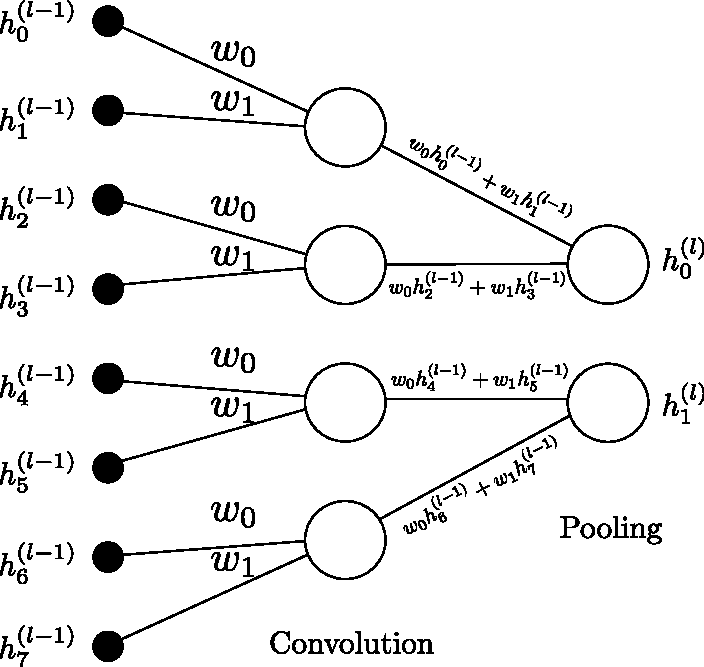
\includegraphics[scale=0.4]{Module 4 (CNN)/pics/Conv_sparse_rep.pdf}\\
    \begin{tiny}Convolution in 1 dimension as sparse connectivity.\end{tiny} 
\end{center}


\begin{itemize}
\item Input $\bh^{(l-1)}$  of dimension 8.
\item Kernel $\bw^{(l)}=\{w_0, w_1\}$. 
\item Stride $s=2$, pooling  $q=2$. 
\end{itemize}

\columnbreak

\begin{itemize}
    \item We need a backpropagation formulation.
    \item A connectivity representation is convenient to make it easy. 
    \item Equivalent connection matrix:
\end{itemize} 
\begin{equation}
    \mathcal{W}^{(l)}=\left(
    \begin{array}{cccc}
    w_0 & 0 & 0 & 0\\
    w_1 & 0 & 0 & 0\\
    0& w_0 &  0 & 0\\
    0& w_1 &  0 & 0\\
    0 & 0 & w_0&  0\\
    0 & 0 & w_1&  0\\
    0 & 0 & 0 & w_0\\
    0 & 0 & 0 & w_1\\
    \end{array}
    \right)
\end{equation}
\end{multicols}
\end{frame}

\begin{frame}{Interpretation as neural connectivity}
\begin{multicols}{2}
\begin{itemize}
\item The first layer is the input
\item The connections  represent the convolution. 
\item $\left\lfloor\frac{M_I+p-M_w+s}{s}\right\rfloor = 4$ 
\item The connection between layers 2 and 3 is the pooling. 
\item The convolution can be computed as $${\mathcal{W}^{(l)}}^\top\bh^{(l-1)}$$
\end{itemize}
\columnbreak
\begin{center}
    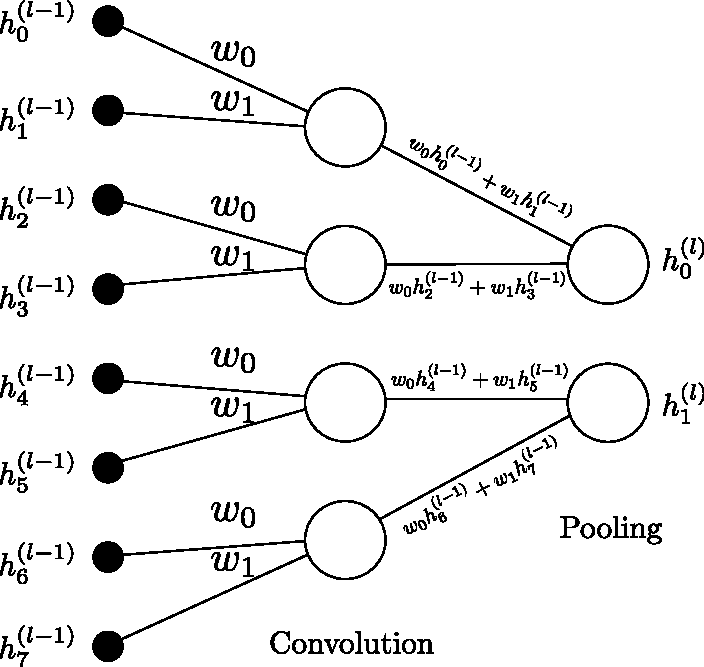
\includegraphics[scale=0.4]{Module 4 (CNN)/pics/Conv_sparse_rep.pdf}\\
    \begin{tiny}Convolution in 1 dimension as sparse connectivity.\end{tiny} 
\end{center}
\end{multicols}
Now, this new sparse connectivity notation can be used to \emph{interpret} the backpropagation. 
\end{frame}

\begin{frame}{Backpropagation in CNN}
\begin{itemize}
    \item Assume a CNN structure  that gives an output $\bo$.
    \item Compute the gradient of the cost function wrt last  kernel $\bW^{(l)}_{j,k}$. 
    \item We can represent the output as:
 \end{itemize}
 
    \begin{equation}
    \bo = \bo\left({\bW^{(L)}}^\top\bphi\left(\cdots{\bW^{(l+1)}}^\top\bvarphi\left(\sum_{j=0}^{C^{(l-1)}-1} \bW^{(l)}_{j,k} * \bH^{(l-1)}_j[n] \right)\right)\right)
\end{equation}

\begin{itemize}
\item All channels other than $k$ and the biases have been ignored since they do not appear in the gradient wrt $\bW^{(l)}_{j,k}$. 
\item Activation $\bvarphi$ flattens the convolution to input  dense layer $l+1$. 
\end{itemize}
\end{frame}

\begin{frame}{Backpropagation in CNN}
\begin{itemize}
\item Now, we assume that the convolution can be changed by some sparse connectivity matrix
\end{itemize}

\begin{equation}
    \bo = \bo\left({\bW^{(L)}}^\top\bphi\left(\cdots{\bW^{(l+1)}}^\top\bvarphi\left(\sum_{j=0}^{C^{(l-1)}-1} \mathcal{W}^{(l)}_{j,k}  \bH^{(l-1)}_j[n] \right)\right)\right)
\end{equation}


\begin{itemize}
    \item And now the formulation is formally identical to the one of a dense neural network. 
    \item Two differences
    \begin{enumerate}
        \item Some matrices (the convolutions) are sparse.
        \item The outputs of the layers are matrices rather than vectors. Therefore, the backpropagated error is a matrix. Instead of $\delta$, we will call it $\Delta$. 
    \end{enumerate}
\end{itemize}
\end{frame}
\begin{frame}{Backpropagation in a CNN}

\begin{itemize}
\item The backpropagation can the be derived in the same way as in Module 1 for a multilayer perceptron:
\begin{equation}\label{eq:bp_update_CNN}
    \mathcal{W}^{(l-1)}_{j,k} \leftarrow  \mathcal{W}^{(l-1)}_{j,k} - \mu   {\bH^{(l-2)}} {{\boldsymbol \Delta}^{(l-1)}}^\top - \mu \lambda \mathcal{W}^{(l-1)}_{j,k}
\end{equation}
with the definition  
\begin{equation}\label{eq:general_error_term_CNN}
    {\boldsymbol \Delta}^{(l-1)} = \mathcal{W}_{j,k}^ {(l)}{\boldsymbol \Delta}^{(l)}\odot
    \varphi'\left(\bZ^{(l-1)}\right)
\end{equation}
\item But sparse matrix $\mathcal{W}_{j,k}^ {(l)}$ represents a convolution.
\end{itemize}
\end{frame}

\begin{frame}{Backpropagation in a CNN}
    \begin{itemize}
        \item  Therefore we can write 

\begin{equation}\label{eq:bp_update_CNN2}
    \bW^{(l-1)}_{j,k} \leftarrow  \bW^{(l-1)}_{j,k} - \mu   {\bH^{(l-2)}} {{\boldsymbol \Delta}^{(l-1)}}^\top - \mu \lambda \bW^{(l-1)}_{j,k}
\end{equation}
with the definition  
\begin{equation}\label{eq:general_error_term_CNN2}
    {\boldsymbol \Delta}^{(l-1)} = \bW_{j,k}^ {(l)}*{\boldsymbol \Delta}^{(l)}\odot
    \varphi'\left(\bZ^{(l-1)}\right)
\end{equation}
    \end{itemize}
\end{frame}

\end{document}

\begin{frame}{What is a convolutional layer}
\begin{center}
    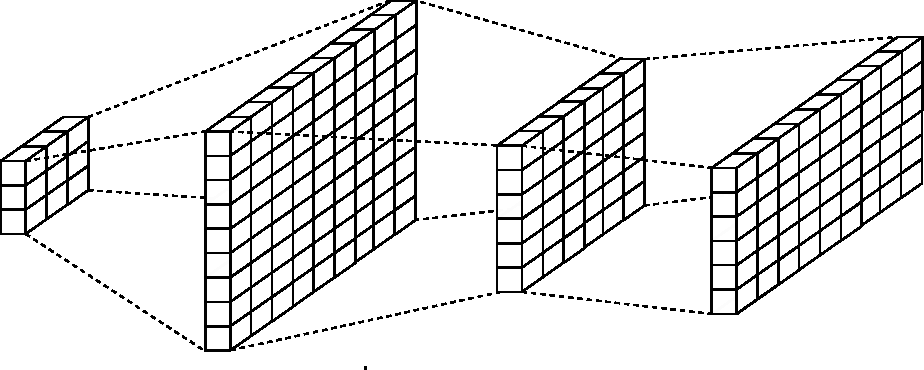
\includegraphics[scale=0.5]{Module 4 (CNN)/pics/f4.4.pdf}
\end{center}
We need a 4 order tensor $\bW$ (a glorified 4D matrix) to map from one image to the other. Think of it as a  bunch of numbers with 4 indexes $w_{i,j,k,l}$:

$$
h_{i,j} = \sum_{k,l} w_{i,j,k,l} x_{k,l}
$$

Indexes $k,l$ match the dimension of the input, and indexes $i,j$ arbitrarily to the hidden image. 

\end{frame}

\begin{frame}{Now, rearrange things}
   We can rearrange the positions of tensor $\bW$  and call it  $\bV$ again.\\
$$
h_{i,j} = \sum_{k,l} w_{i,j,k,l} x_{k,l} = \sum_{a,b} v_{i,j,a,b} x_{i+a,j+b} 
$$
where $k=i+a, l=j+b$ for certain limits in $a$ and $b$.

Recall that $\bW$ is arbitrary, so both operations are equivalent.

\end{frame}

\begin{frame}{Apply translation invariance}

We want the resulting image translation invariant:
\begin{itemize}
\item A shift $\bX$ translates into a  shift in $\bH$. 
\item Thus, the tensor must not depend on the image position:

$$
h_{i,j} = \sum_{a,b} v_{a,b} x_{i+a,j+b} 
$$

\item This is a 2D \emph{cross-correlation} operation. Tensors are  matrices now.  \\

\item Convolution and cross-correlation are formally the same operation; in convolution one of the elements is flipped. 
\item But $\bV$ is arbitrary and \emph{convolution} is fancier.   

\end{itemize}



\end{frame}


\begin{frame}{Now, apply locality properties}

We want every pixel of the hidden (destination) image to contain information of a region $\pm \Delta_a$, $\pm \Delta_b$, not the whole image.
\begin{multicols}{2}
\begin{center}
    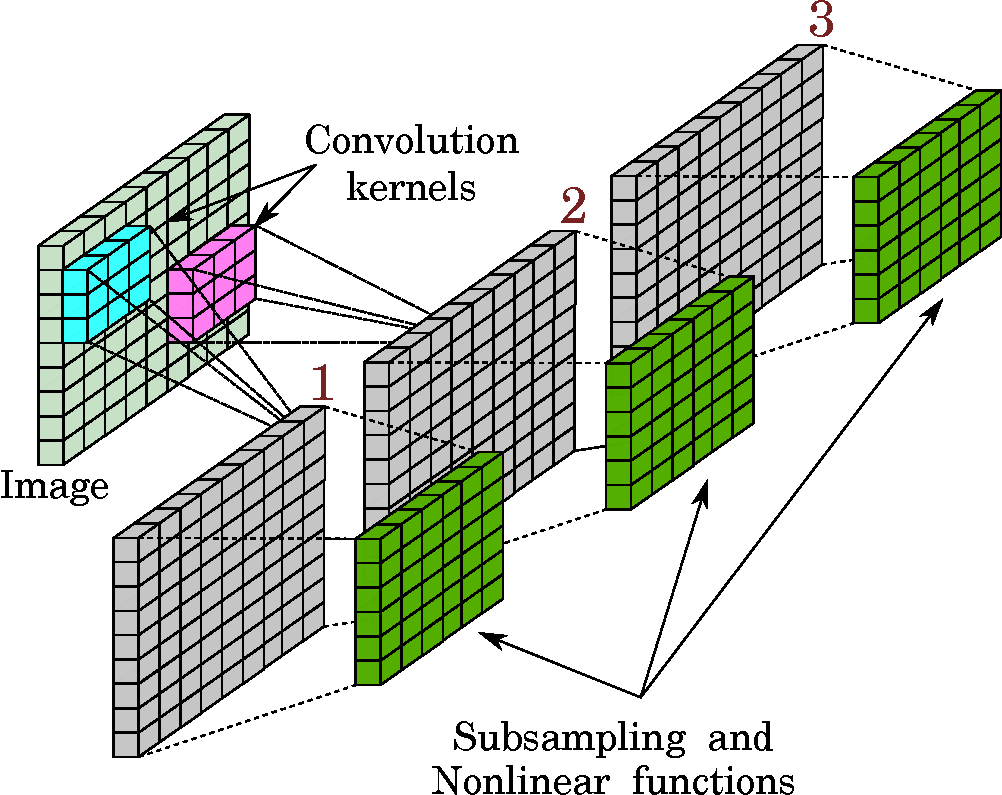
\includegraphics[scale=0.3]{Module 4 (CNN)/pics/f5.4.pdf}
\end{center}
\columnbreak
$$
h_{i,j} = \sum_{a=-\Delta_a}^{\Delta_a}\sum_{b=-\Delta_b}^{\Delta_b} v_{a,b} x_{i+a,j+b} 
$$
We can do it $1 \leq c \leq C$ times: 
$$
h_{i,j,c} = \sum_{a=-\Delta_a}^{\Delta_a}\sum_{b=-\Delta_b}^{\Delta_b} v_{a,b,c} x_{i+a,j+b}
$$
And \emph{voil\`a} two (3D) tensors again.

\end{multicols}

After this, we can apply nonlinearities and reductions to the images.
    
\end{frame}

\begin{frame}{Channels}
\begin{itemize}
\item The paths from the original image to the convolution outputs are calle \emph{channels}. 

\item We can apply the convolution again to all the channel outputs. 
\item The convolution operator maps from a 3D tensor to a 3D tensor  

$$
h^{(2)}_{i,j,c} = \sum_{a=-\Delta_{a,c}}^{\Delta_{a,c}}\sum_{b=-\Delta_{b,c}}^{\Delta_{b,c}} v_{a,b,c,d} h^{(1)}_{i+a,j+b,d}
$$

\item An image with $L$ channels and given dimensions  can be mapped to an image with $M$ channels and arbitrary dimensions.  
\end{itemize}    
\end{frame}
\begin{frame}{How does a convolution look like?}
This is a NASA pic of the Cat's Eye nebula. 
    \begin{center}
       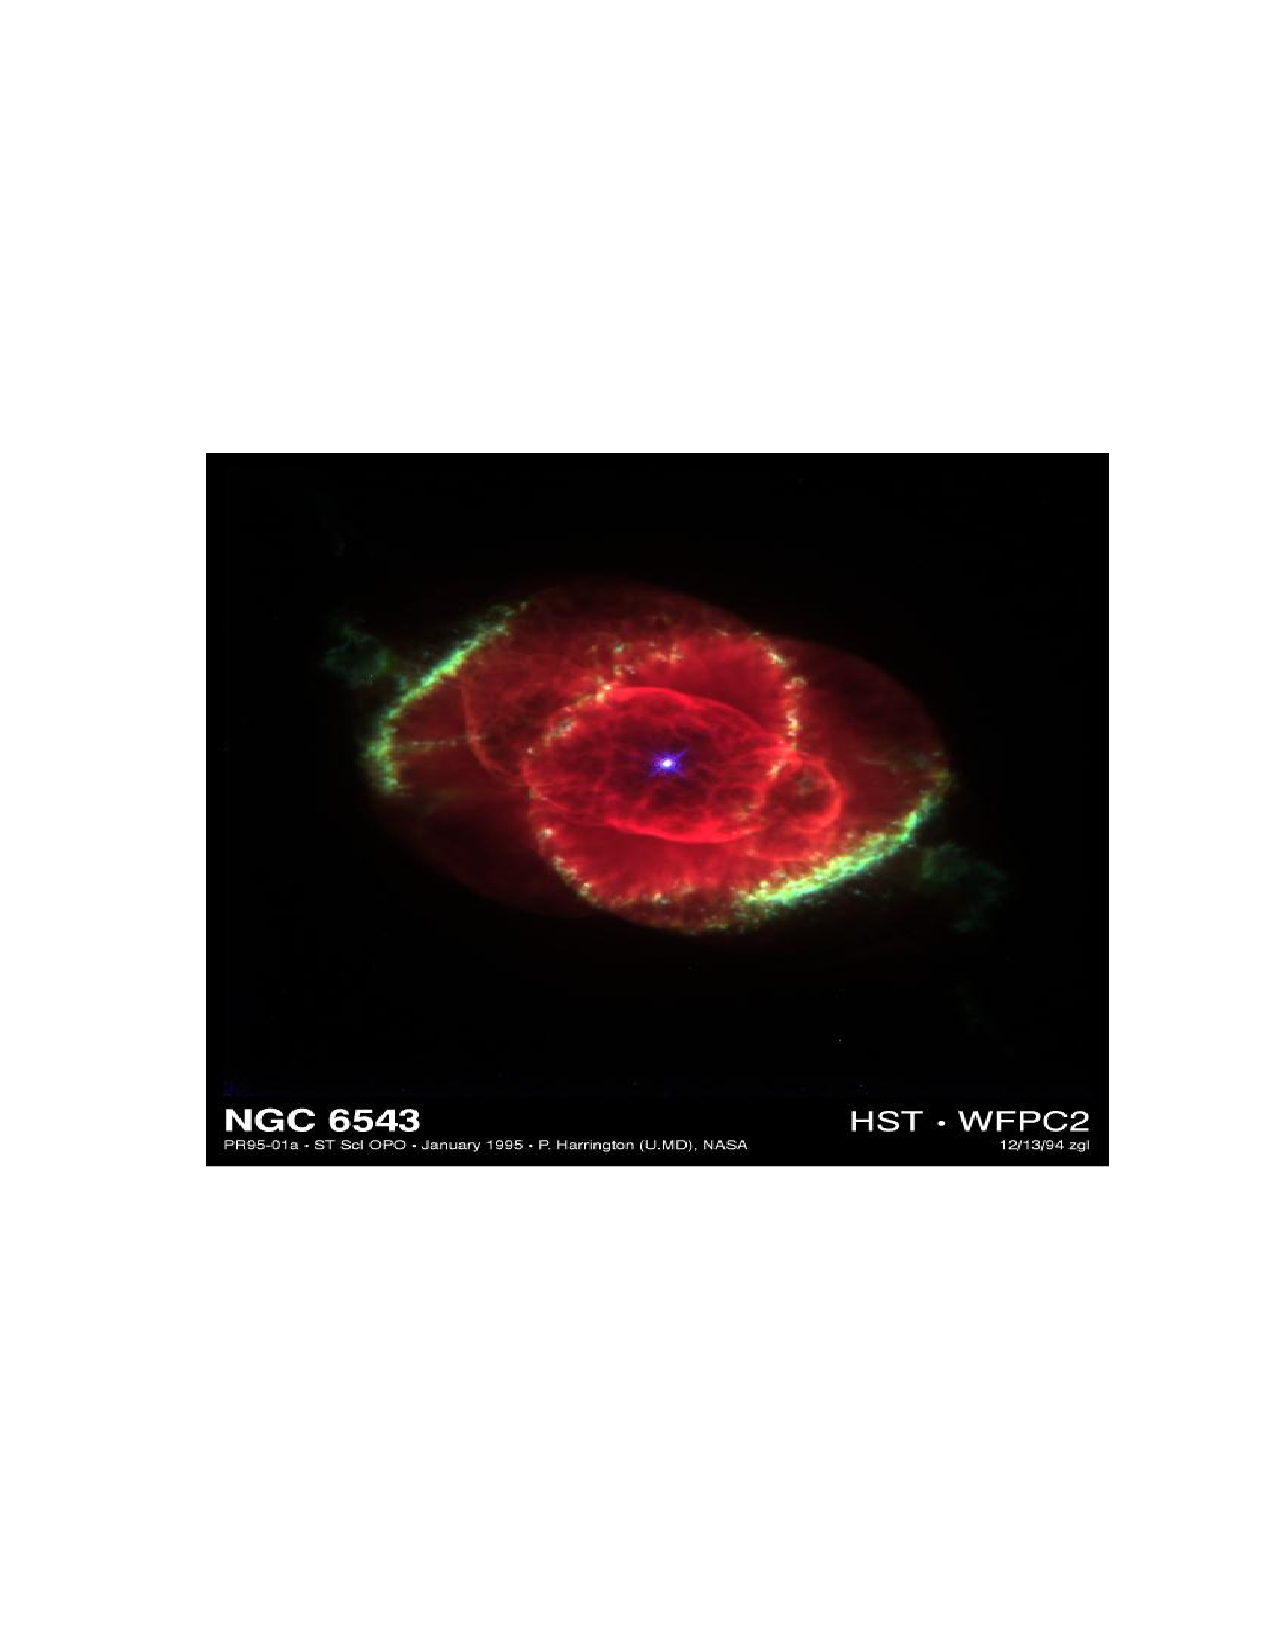
\includegraphics[scale=0.25]{Module 4 (CNN)/pics/NGC6543.pdf} 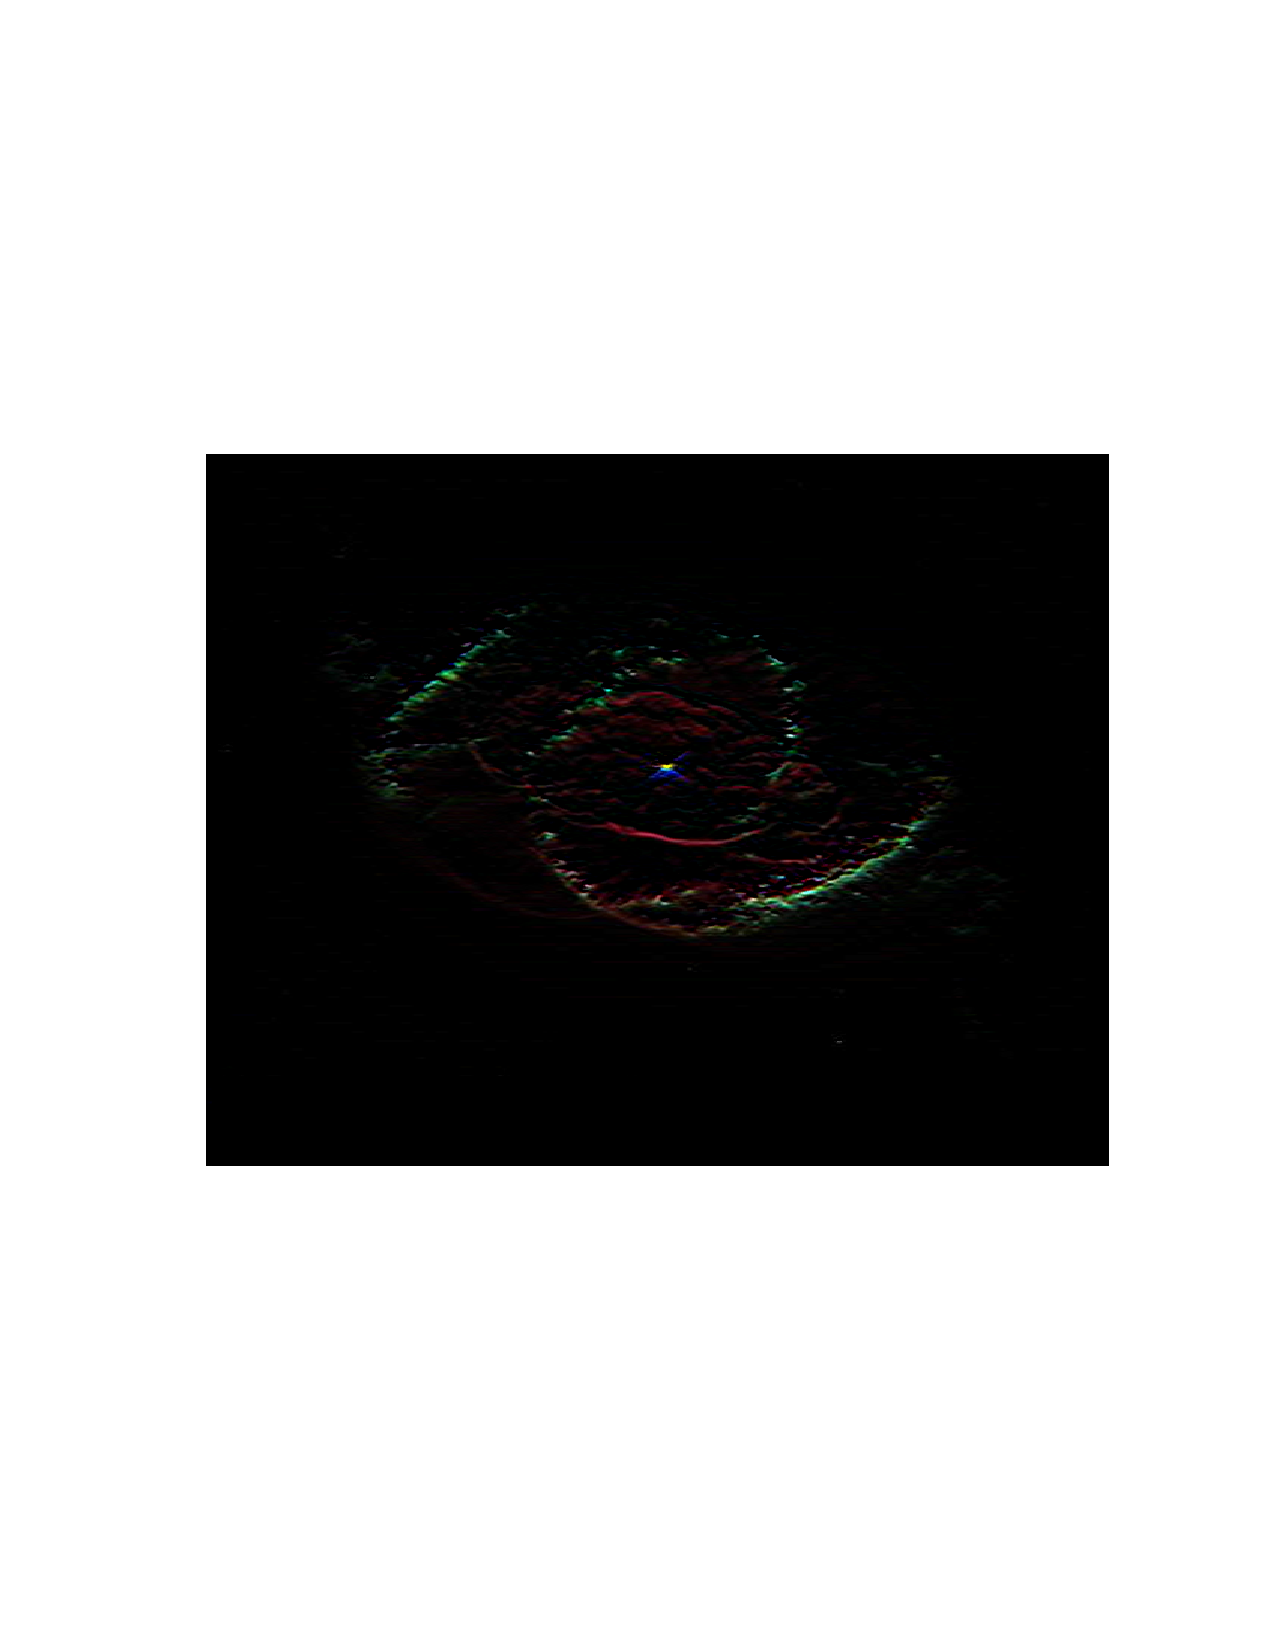
\includegraphics[scale=0.25]{Module 4 (CNN)/pics/NGC6543_h.pdf}
       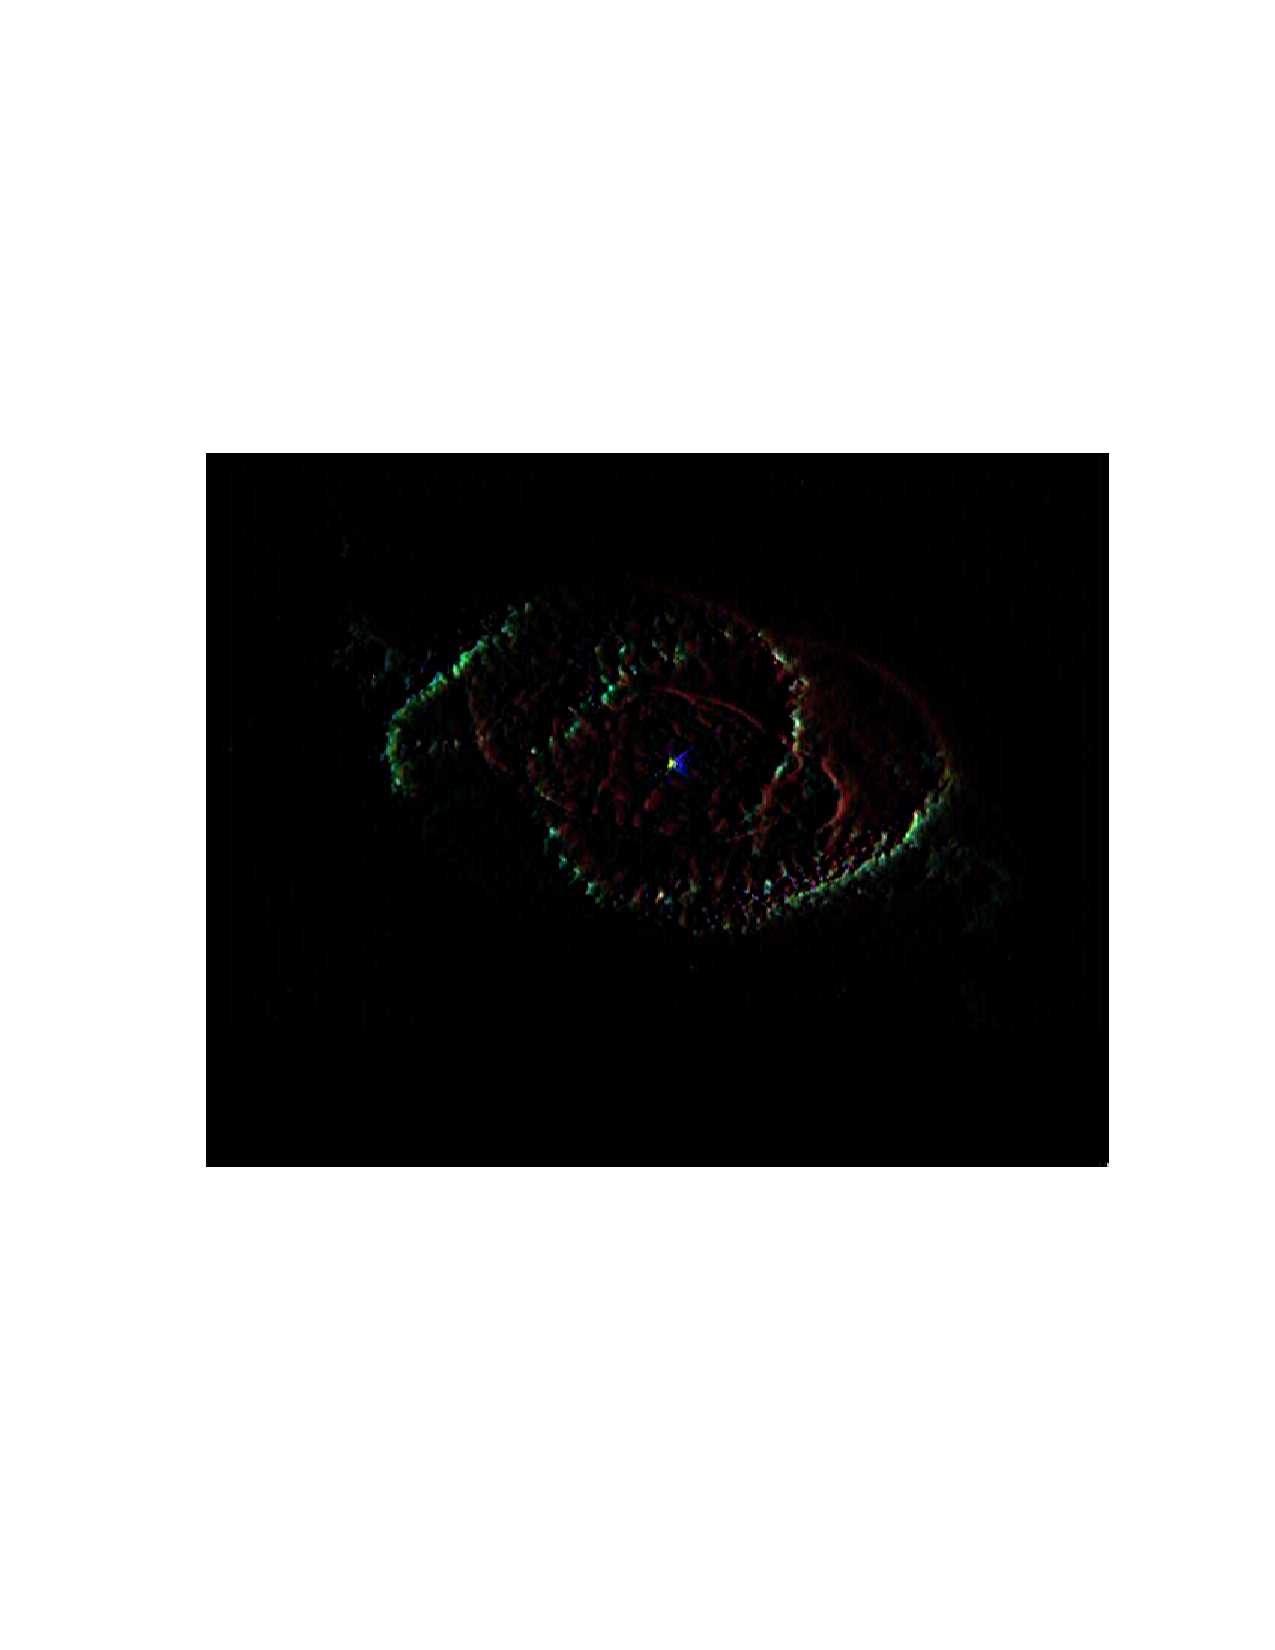
\includegraphics[scale=0.25]{Module 4 (CNN)/pics/NGC6543_v.pdf}
    \end{center}
    We applied two convolutions to each channel of the image, with the \emph{kernels} 
 $$
        \bV_1 = \left( 
        \begin{array}{rrr}
             -1&0&1  \\
             -1&0&1  \\
             -1&0&1  \\
        \end{array}
        \right)
        \text{~~and~~}
        \bV_2 = \left( 
        \begin{array}{rrr}
             -1&-1&-1  \\
             0&0&0  \\
             1&1&1  \\
        \end{array}
        \right)
$$
\end{frame}


\begin{frame}{How does a convolution look like?}
This is a NASA pic of the Cat's Eye nebula. 
    \begin{center}
       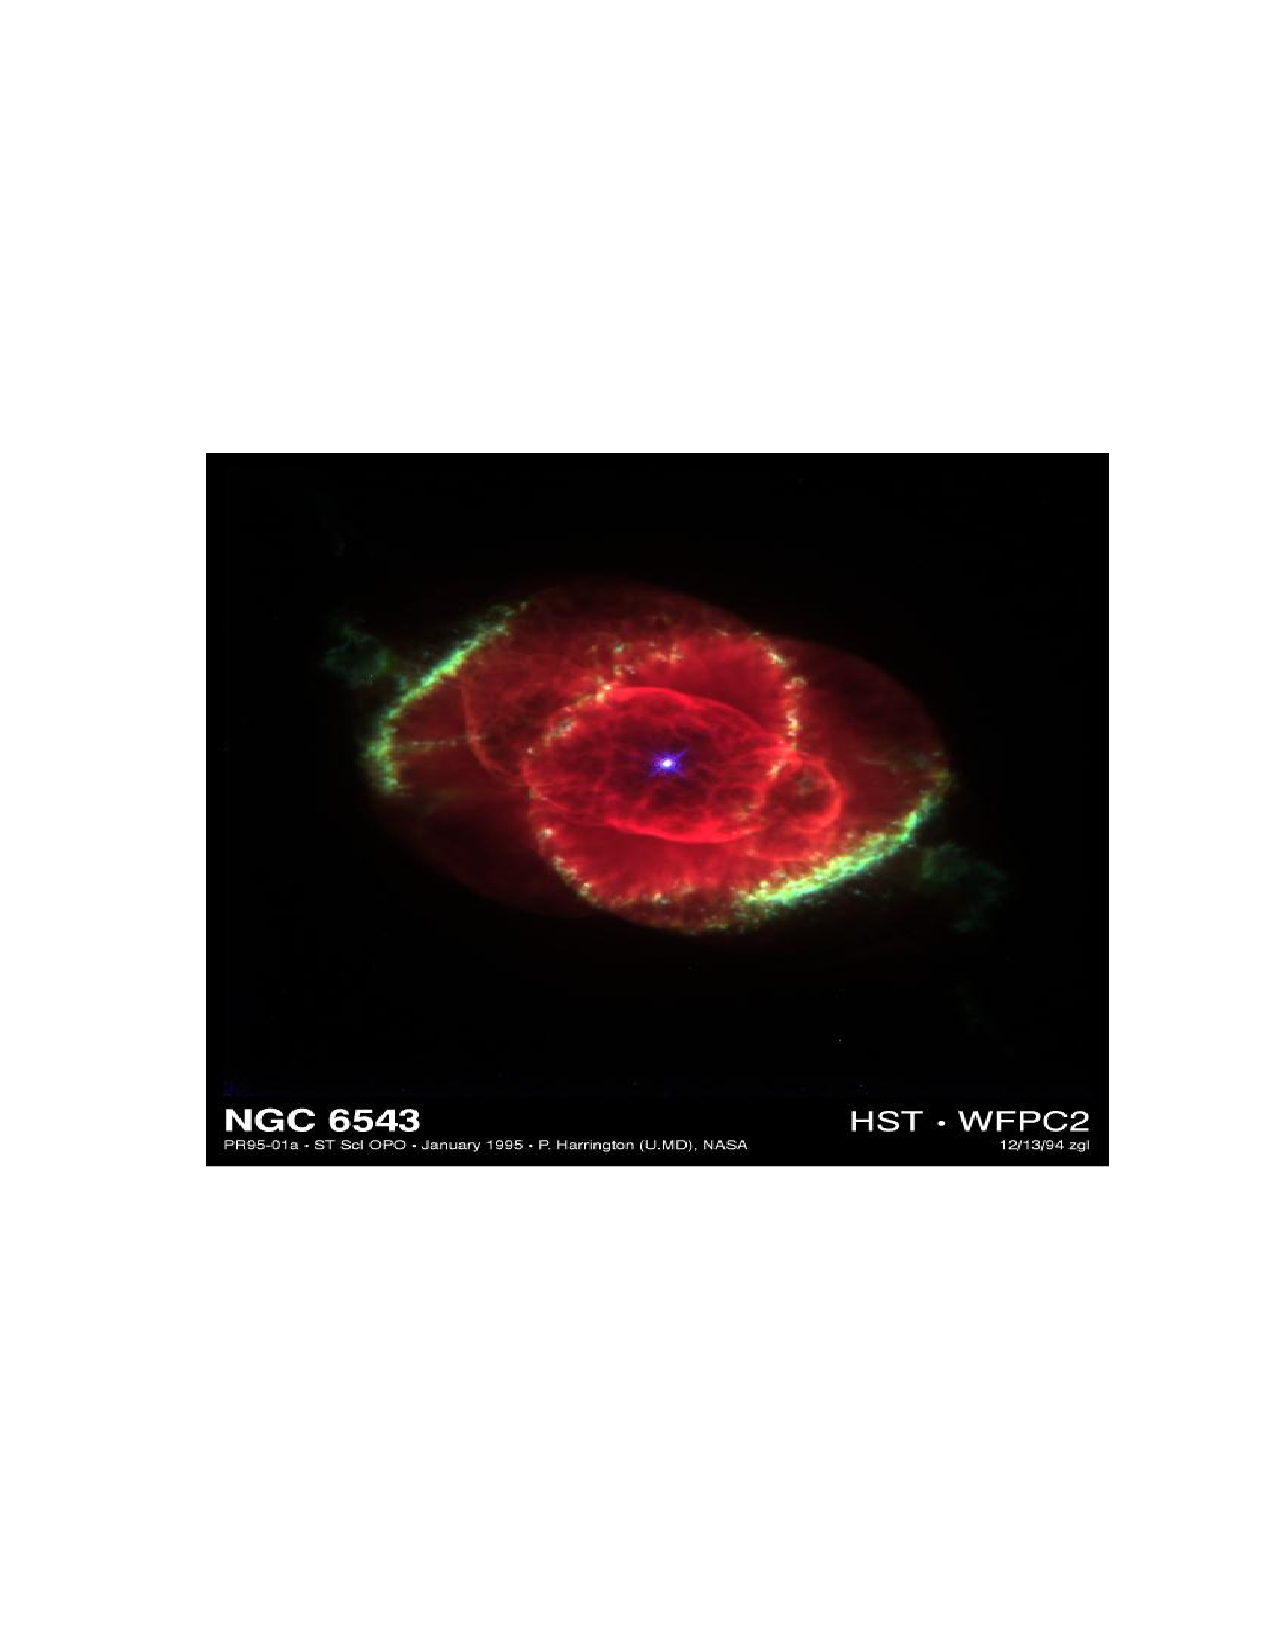
\includegraphics[scale=0.25]{Module 4 (CNN)/pics/NGC6543.pdf} 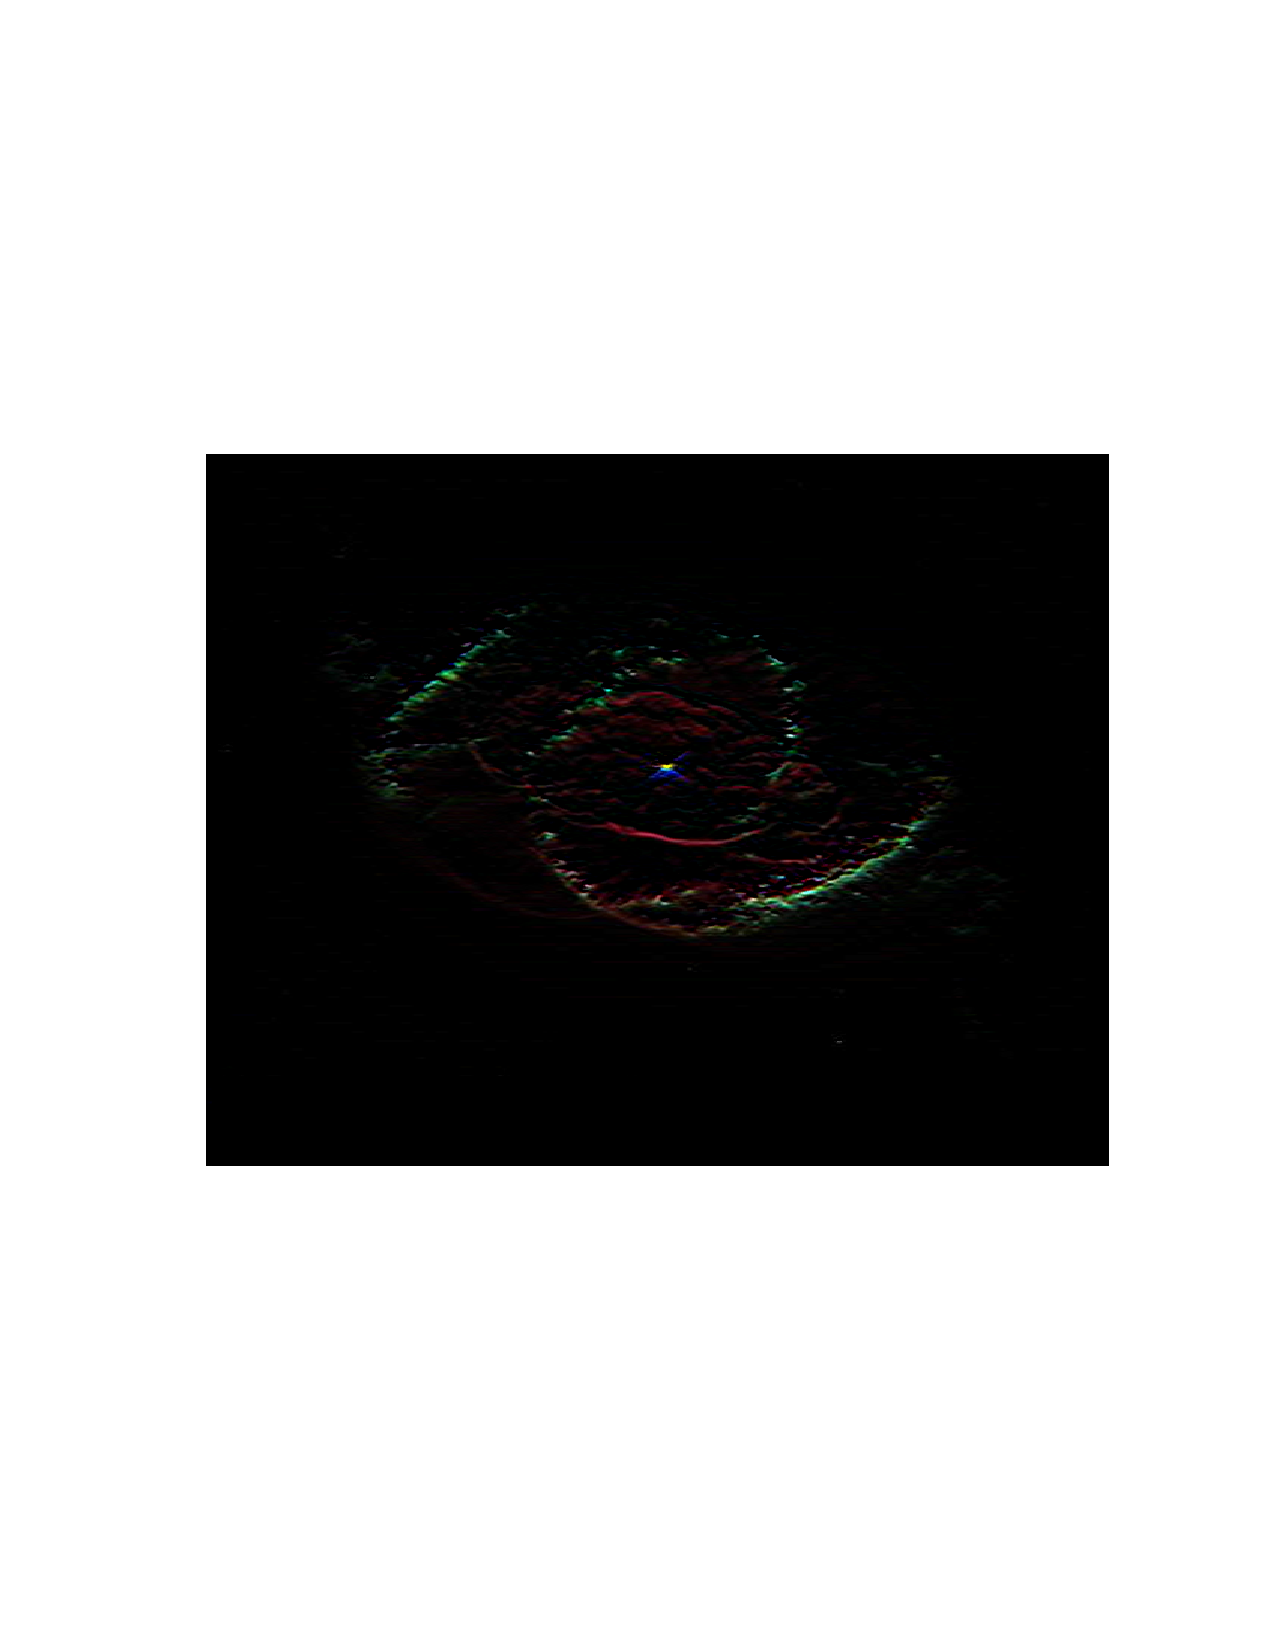
\includegraphics[scale=0.25]{Module 4 (CNN)/pics/NGC6543_h.pdf}
       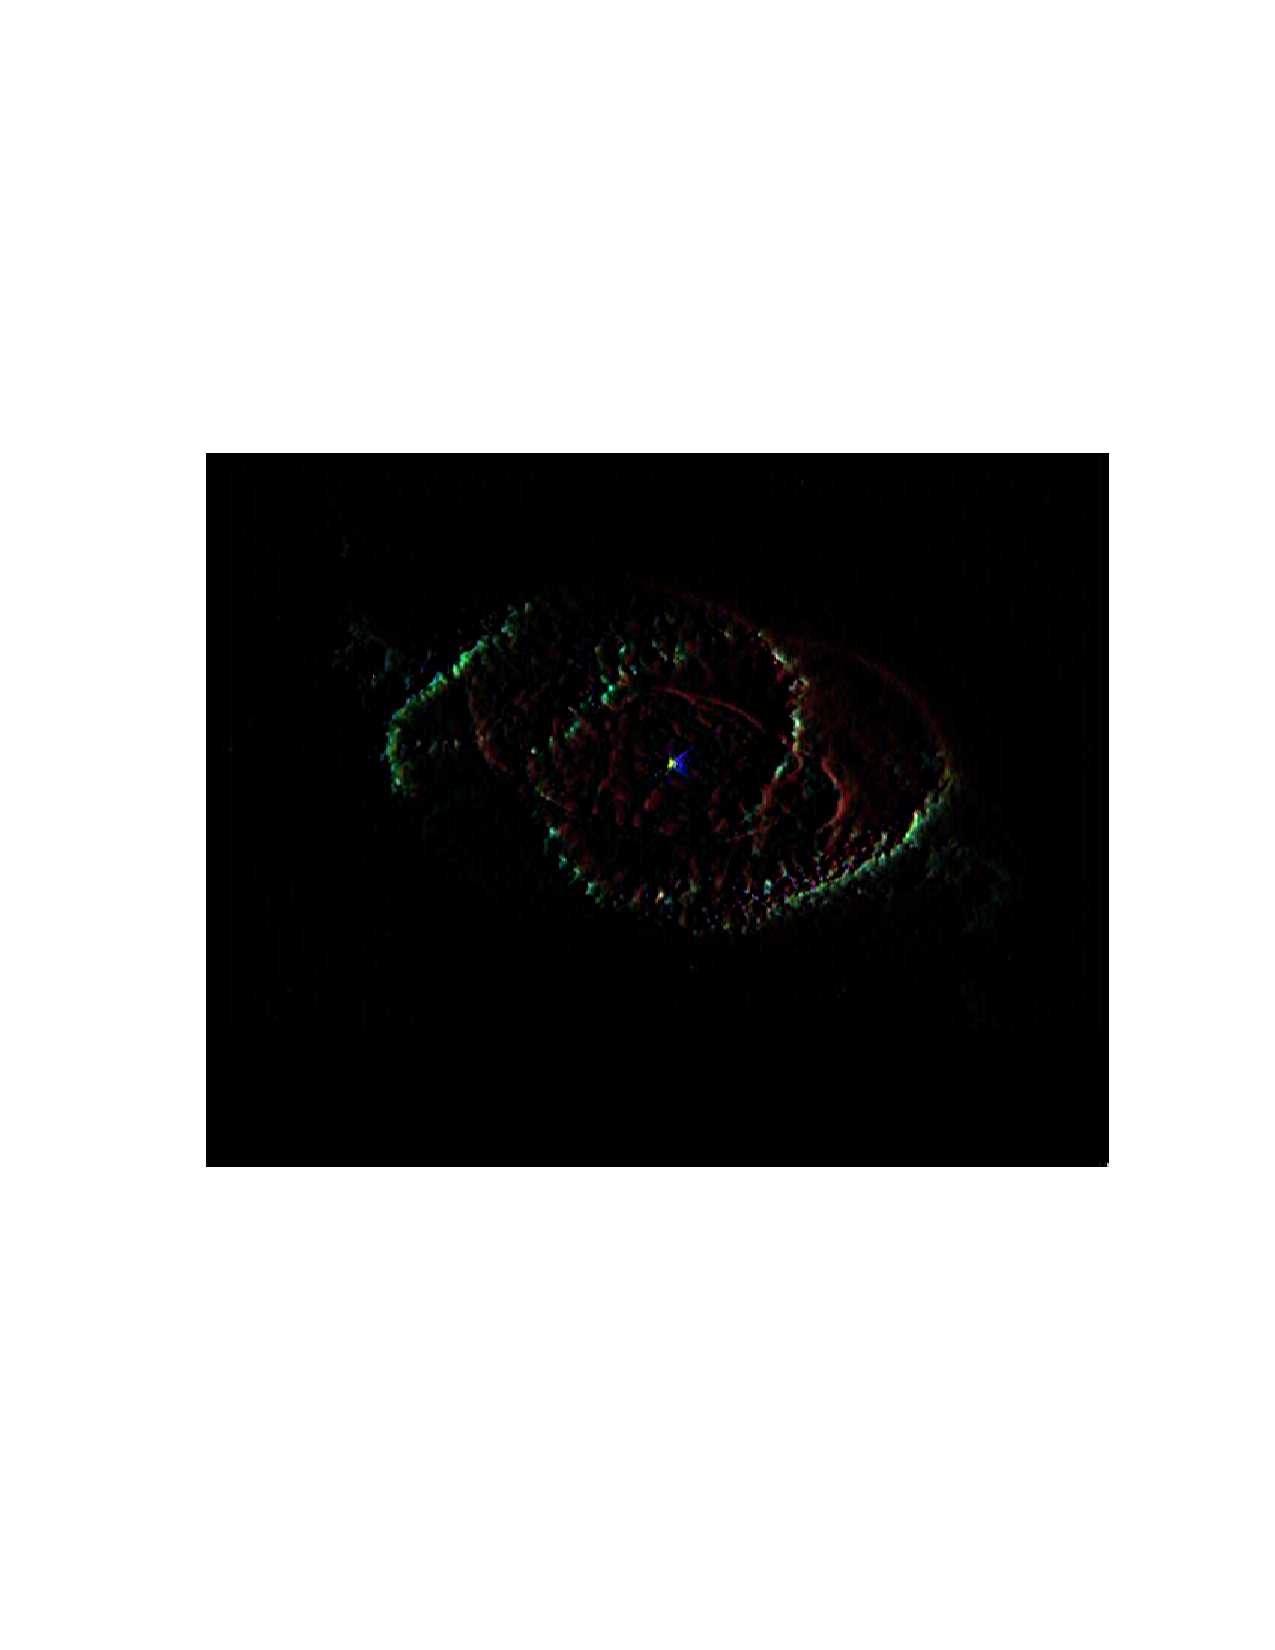
\includegraphics[scale=0.25]{Module 4 (CNN)/pics/NGC6543_v.pdf}
    \end{center}
   We can see that the convolutions reveal two characteristics in both dimensions of the image, which are changes. \\
   Here we actually see a mapping from a 3D image to two 3D images.
   \vspace{2cm}
\end{frame} 

\begin{frame}{Optimizing a kernel}
    \begin{itemize}
        \item The previous example is a particular case of edge detection.
        \item This is done in classical image processing where we want to use edges as features. 
        \item In reality, we do not know what are the features to be extracted and this is why we apply convolutional neural networks.
        \item The convolution kernels are optimized by back propagation under a given criterion. 
    \end{itemize}
    
\end{frame}
\begin{frame}{Optimizing a kernel}
\begin{itemize}
    \item We must recall that a convolutional layer is nothing but a mapping from a tensor $\bH^{(l)}$, which we assume of order 3 to another tensor $\bH^{(l+1)}$ of order 3. 
    
    
    $$
    \bH^{(l)} \in \mathbb{R}^{I,J,D_l} \rightarrow     \bH^{(l+1)} = \text{conv}\left( \bV^{(l)}\bH^{(l)}\right) \in \mathbb{R}^{I,J,D_{j+1}}
    $$
    which is expressed as 
    
    $$
h^{(l+1)}_{i,j,c} = \sum_{a=-\Delta_a}^{\Delta_a}\sum_{b=-\Delta_b}^{\Delta_b} v_{a,b,c,d} h^{(l)}_{i+a,j+b,d}
$$
    
    \item By now, we are ignoring the nonlinear operations between layers. 
    \item In must applications, we want to preserve the dimensions between convolutions, so we crop the images. 
\end{itemize}
\end{frame}


\begin{frame}{Optimizing a kernel}
The optimization needs the derivative of each node output with respect to each coefficient:
$$
\frac{\delta h^{(l+1)}_{i,j,c}}{\delta w_{a,b,c,d}}=h^{(l)}_{i+a,j+b,d}
$$

Notice that when we compute the expectation of the gradient, we will do it across $i,  j$ because a weight is applied to all pixels of the image.

\end{frame}
\begin{frame}{Padding, stride and pooling}

\begin{itemize}
    \item Convolutions have a reduced number of parameters.
    \item Convolutions crop the image.
    \item On the other side, the number of feature maps increase fast.
\end{itemize}
Some operations are common to reduce the impact of these. 
\begin{itemize}
    \item In order to avoid cropping, images are zero padded around them.
    \item In order to reduce the computational cost, stride is often applied, this is, the sliding window of the convolution is applied slid more than one pixel. 
    \item The resolution of the feature maps is reduced by pooling.
    \begin{itemize}
        \item Max Pooling: $max(h_{i-\Delta:i+\Delta,j-\Delta:j+\Delta},c)$.\\ 
        It takes the maximum of non-overlapping submatrices of dimension $\Delta\times\Delta$ of each channel.
        \item Mean Pooling: take the mean of non-overlapping matrices of each channel.  
    \end{itemize}
\end{itemize}


    
\end{frame}

\begin{frame}{Next up...}
\begin{itemize}
    \item The basic convolutional neural network
    \item Python examples of CNNs
    \item A review of more complex CNNs: AlexNet, VGG16, NiN nets.
    \item Basics on how to program them.
\end{itemize}
    
\end{frame}

\end{document}	




Convolutional Neural Networks
Elements of a CNN
    Overall structure of a CNN
    Convolutions
    Convolutions in 2 dimensions 
    Padding
    Stride
    Pooling
    Formulation of the convolution layer in a CNN
    Backpropagation of a convolution layer
Operational elements of CNN
    Regularization techniques
    Normalization techniques
    Optimizers
Extensions of the CNN
    AlexNet
    VGG
    Inception
    ResNet
    Xception
    MobileNet
    DenseNet
    EfficientNet
Transfer learning for CNN extensions
